% \pagebreak[4]
% \hspace*{1cm}
% \pagebreak[4]
% \hspace*{1cm}
% \pagebreak[4]

\chapter{Phân tích thiết kế xây dựng hệ thống} \label{design-analysis}

\ifpdf
    \graphicspath{{DesignAnalysis/Chapter1Figs/PNG/}{DesignAnalysis/Chapter1Figs/PDF/}{DesignAnalysis/Chapter1Figs/}}
\else
    \graphicspath{{DesignAnalysis/Chapter1Figs/EPS/}{DesignAnalysis/Chapter1Figs/}}
\fi

\section{Phân tích tổng quát hệ thống}
Các yêu cầu của hệ thống:
\begin{itemize}
	\item Cung cấp các phương pháp để xác định được trình độ, nguyện vọng và các yếu tố ưu tiên khác trong việc học tiếng Anh của người dùng thông qua giao diện đơn giản, dễ tương tác. Qua đó, đưa ra được các kết quả tư vấn là tài liệu, sách, video, bài giảng Tiếng Anh..v..v... tương ứng.
	\item Cung cấp giao diện quản lý cho quản trị viên dễ dàng thực hiện các thao tác quản lý thông tin người dùng, quản lý hệ cơ sở tri thức gồm tập câu hỏi kiểm tra và tài liệu tiếng Anh.
\end{itemize}
Qua việc khảo sát các hệ thống tư vấn đã và đang được triển khai, đồng thời để giải quyết các yêu cầu đặt ra ở trên, hệ thống đề xuất xây dựng trong đề tài này sẽ có cấu trúc gồm các thành phần sau:

\begin{itemize}
	\item \textbf{Module xác định trình độ:} có nhiệm vụ xác định trình độ của người sử dụng, thông qua việc thực hiện bài kiểm tra General English Test . Sử dụng kĩ thuật Computerized Adaptive Testing, các câu hỏi đưa ra cho người dùng sẽ được tuỳ biến sao cho độ khó phù hợp với năng lực của người dùng. Nhờ vậy, số lượng câu hỏi mà người dùng cần trả lời để xác định được trình độ của họ là ít hơn bài kiểm tra truyền thống, song vẫn cho ra kết quả chính xác như tương tự. Kết quả của bước này sẽ cho ra User level bao gồm trình độ đọc hiểu, vốn từ vựng và vốn ngữ pháp.
	\item \textbf{Module xác định nguyện vọng:} có nhiệm vụ nhận input về nguyện vọng từ người dùng, cụ thể là chủ đề mà người dùng muốn học. Có thể đưa ra các gợi ý cho người dùng về các chủ đề phổ biến. Kết quả bước này sẽ cho ra User preference là các chủ đề người dùng muốn học dưới dạng keyword.
	\item \textbf{Context-matching:} thực hiện nhận thông tin User level và User preference tổng hợp thành User profile. Sau đó sử dụng thuật toán Context-matching tiến hành matching với profile tài liệu và trả về những kết quả có độ khớp cao nhất.
	\item \textbf{Kansei:} kết quả sau khi Context Matching sẽ được trả về cho người dùng đánh giá trên thang cảm xúc từ "rất thích" cho đến "rất ghét". Dựa vào đánh giá, những thuộc tính trong profile tài liệu ứng với "thích" sẽ được cập nhập vào User preference và lấy nó làm cơ sở context matching các kết quả tiếp theo.
	\item \textbf{Hệ cơ sở tri thức:} sử dụng cơ sở dữ liệu online của Firebase làm cơ sở tri thức cho hệ thống. Nhiệm vụ của nó là trao đổi thông tin với client, cập nhập thông tin mới đảm bảo tính đồng bộ cho toàn hệ thống. \\Dữ liệu được lưu trữ bao gồm:
		\begin{itemize}
			\item Dữ liệu câu hỏi và đáp án General English Test
			\item Thông tin người dùng : id, loại người dùng, trình độ, nguyện vọng.
			\item Dữ liệu tài liệu học Tiếng Anh: tên, loại tài liệu, tác giả, miêu tả, nội dung ..v..v... và profile của tài liệu dưới dạng một tập keyword.
		\end{itemize}
\end{itemize}

Sau đây là mô hình kiến trúc của ứng dụng:

\begin{figure}[H]
  \begin{center}
    %\leavevmode
    \ifpdf
      \includegraphics[scale=0.5]{appflow}
    \else
      \includegraphics[scale=0.5]{appflow}
    \fi
    \caption{Mô hình kiến trúc ứng dụng}
    \label{Appflow}
  \end{center}
\end{figure}

\section{Xây dựng hồ sơ người dùng}
User profile bao gồm trình độ và nguyện vọng của người dùng. Những thông tin này sẽ được dùng trong quá trình matching với các tập dữ liệu bằng thuật toán Context-matching . \\

\begin{figure}[H]
  \begin{center}
    %\leavevmode
    \ifpdf
      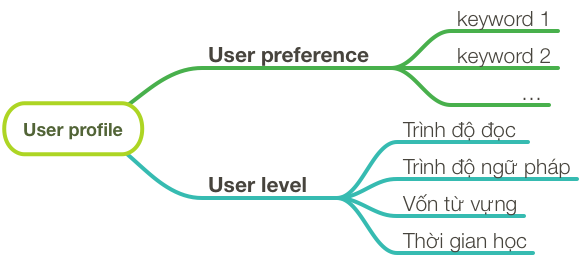
\includegraphics[scale=0.7]{userprofile}
    \else
      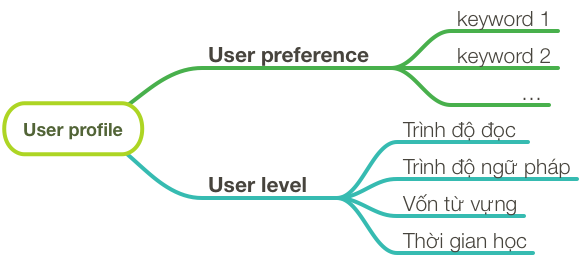
\includegraphics[scale=0.7]{userprofile}
    \fi
    \caption{User profile}
    \label{Userprofile}
  \end{center}
\end{figure}

\subsection{Xác định trình độ người dùng}

Để xác định trình độ Tiếng Anh của người dùng, tất cả các khía cạnh sau đây cần được khai thác:
\begin{itemize}
\item Thời điểm bắt đầu học
\item Trình độ đọc hiểu
\item Trình độ ngữ pháp
\item Vốn từ vựng
\end{itemize}

Bài kiểm tra tương tác CAT sẽ được sử dụng để đánh giá trình độ.Phương thức chọn câu hỏi và đánh giá bài thi CAT trong đề tài được xây dựng dựa trên mô hình Thử tỉ lệ xác suất nối tiếp \cite{welchfrick} (Sequential probability ratio test).\\ 

Nguyên lý căn bản nằm bên trong mô hình này là xác suất hợp lý rời rạc. Giả sử từ quan sát thực tế cho thấy thí sinh có trình độ tiếng Anh xuất sắc đạt trung bình 85/100 điểm trong bài thi, trong khi thí sinh có trình độ thấp chỉ đạt 35/100 điểm. Dưới góc nhìn hệ thống có thể coi nó như tập luật $if....else$ sau đây:

\begin{enumerate}
	\item Thí sinh có trình độ xuất sắc, đã nắm vững kiến thức và hiểu rõ câu hỏi cũng như phương pháp giải quyết, do vậy khả năng mà họ trả lời đúng câu hỏi sẽ là 85 \%. 
		\subitem Prob(Correct|Master) = .85 ($P_m$)
		\subitem Prob(Incorrect|Master) = .15
	\item Ngược lại, thí sinh có trình độ thấp, trả lời phần lớn dựa trên may rủi, giác quan thứ 6 của bản thân, do vậy khả năng mà họ trả lời đúng câu hỏi sẽ là 35 \%. 
		\subitem Prob(Correct|Nonmaster) = .35 ($P_n$)
		\subitem Prob(Incorrect|Nonmaster) = .75
\end{enumerate}  

Trong bài kiểm tra CAT, với câu hỏi bất kì phù hợp trình độ được chọn ra trong tập câu hỏi đưa cho thí sinh. Quan sát trả lời của thí sinh, xác suất khả năng trình độ sẽ được tính bằng:

\begin{equation}
PR = \dfrac{P_m^t(1-P_m)^f}{P_m^t(1-P_m)^f}
\end{equation}
trong đó $P_m = $ khả năng thí sinh trình độ xuất sắc trả lời đúng câu hỏi

$P_n = $ khả năng thí sinh trình độ thấp trả lời đúng câu hỏi

$t = $ tổng số câu hỏi thí sinh trả lời đúng 

$f = $ tổng số câu hỏi thí sinh trả lời sai 

Giá trị $PR$ sau đó sẽ được đem so sánh với tập luật:

\begin{center}
\fbox{\begin{minipage}{0.9\textwidth}
\begin{itemize}
	\item Nếu $PR > UBN$ (Upper Bound Nonmastery: giá trị ngưỡng trên của độ không thuần thục) -> trình độ người dùng thấp hơn câu hỏi hiện tại, chọn câu hỏi tiếp theo ở trình độ thấp hơn để tiếp tục đánh giá .
	\item Nếu $PR < LBM$ (Lower Bound Mastery: giá trị ngưỡng dưới của độ thuần thục) -> trình độ người dùng nằm trên câu hỏi hiện tại, chọn câu hỏi tiếp theo ở trình độ cao hơn để tiếp tục đánh giá. 
	\item Nếu $UBN < PR < LBM$, kết quả hiện tại chưa đủ để đánh giá trình độ người dùng, chọn câu hỏi tiếp theo ở cùng trình độ để tiếp tục đánh giá.  
\end{itemize}
\end{minipage}}
\end{center}


Trình độ của thí sinh được xác định khi $PR$ lớn hơn giá trị $UBN$ hoặc nhỏ hơn giá trị $LBM$. Tuy nhiên, xét trong trường hợp thực tế có khả năng xảy ra việc số lượng câu hỏi thí sinh trả lời sai bằng với số lượng câu hỏi thí sinh trả lời đúng. Điều này dẫn đến tình trạng thí sinh trả lời một số lượng lớn câu hỏi nhưng vẫn không xác định được trình độ. Điều kiện dừng sẽ được đưa vào để giải quyết trường hợp đó.

Hệ thống sẽ dừng bài kiểm tra đánh giá nếu như:
\begin{itemize}
	\item Nếu $PR > UBN$ và \textit{"độ khó hiện tại là thấp nhất"}
	\item Nếu $PR < LBM$ và \textit{"độ khó hiện tại là cao nhất"}
	\item Nếu $UBN < PR < LBM$ và số lượng câu hỏi hiện tại vượt \textit{ngưỡng câu hỏi}
\end{itemize}

Sau dây là mô hình đánh giá trình độ người dùng sử dụng trong đề tài:

\begin{figure}[H]
  \begin{center}
    %\leavevmode
    \ifpdf
      \includegraphics[scale=0.8]{cat}
    \else
      \includegraphics[scale=0.8]{cat}
    \fi
    \caption{Mô hình bài kiểm tra tương tác}
    \label{CATModel}
  \end{center}
\end{figure}

Trước tiên, trình độ ban đầu của người dùng sẽ được xác định qua câu hỏi "Bạn đã học tiếng Anh được bao lâu rồi". Trình độ của một người nào đó thường tỉ lệ thuận với thời gian họ bỏ ra để học.  do vậy ta có thể phần nào phán đoán được thông qua thông tin thời gian học. Đây là bước tiền đề trước khi đi vào thực hiện bài thi.\\

Tập câu hỏi đánh giá trình độ ban đầu, gồm hơn 70 câu hỏi lấy từ trang \url{http://www.englishjet.com/}. Hình thức của câu hỏi ở dạng trắc nghiệm với 4 đáp án. Chúng được phân loại vào từng tập câu hỏi khác nhau theo các \textit{chủ đề}\{\textit{đọc hiểu, từ vựng, ngữ pháp}\} và \textit{trình độ}\{\textit{nhập môn, cơ bản, trung bình, khá, cao cấp}\}. Dựa trên trình độ hiện tại của người dùng, hệ thống sẽ chọn bất kì một câu hỏi trong tập câu hỏi cùng trình độ ra để kiểm tra. Sau khi kết thúc một chủ đề, trình độ hiện tại của người dùng sẽ được sử dụng làm trình độ ban đầu trong đánh giá chủ đề tiếp theo. \\

\textbf{You can exchange the gift ......}\\
  \begin{choices}
    \choice so long that
    \choice while
    \choice as long as
    \choice meanwhile
    \choice whether
  \end{choices}
\begin{flushright}{\textbf{...... it is returned within seven days.}}\\	
\end{flushright}

 Việc đánh giá kết quả được thực hiện theo tập luật đã đề cập ở phía trên. Dựa vào quan sát thử nghiệm trong thực tế, hệ thống đề xuất trong đề tài sử dụng các giá trị $UBN = 0.02$, $LBM = 7$ và \textit{ngưỡng câu hỏi} $= 5$.\\
 
 Ví dụ, một thí sinh học tiếng Anh được 4 năm làm bài kiểm tra trình độ. Hệ thống sẽ dự đoán trình độ của anh ta nằm ở mức trung bình và đưa ra câu hỏi ở mức trình độ đó. Bắt đầu với chủ đề \textit{từ vựng}, thí sinh này trả lời đúng liên tiếp 3 câu hỏi. $PR$ của anh ta lúc đó sẽ là $\dfrac{0.85^3(1-0.85)^0}{0.35^3(1-0.35)^0}\: \approx \: 14.3236 > LBM = 7$. Điều kiện tăng trình độ thoả mãn, trình độ thí sinh được nâng lên mức khá. Tiếp tục quá trình đánh giá, lần này với câu hỏi trình độ khá, thí sinh lần lượt đạt kết quả Đúng-Sai-Đúng-Đúng-Sai, tương ứng với $PR = \dfrac{0.85^3(1-0.85)^2}{0.35^3(1-0.35)^2}\: \approx \: 3.305 $. Do $ UBN < PR < LBM $ và số lượng câu hỏi đã trả lời đạt ngưỡng, việc đánh giá trình độ \textit\textbf{từ vựng} của thí sinh kết thúc. Kết quả là thí sinh đạt trình độ \textbf{\textit{khá}} về \textit{từ vựng}. Lấy trình độ \textit{khá} làm trình độ ban đầu, hệ thống tiếp tục đánh giá chủ đề tiếp theo. Kết quả thu được là \textbf{\textit{trung bình}} về \textit{ngữ pháp} và \textbf{\textit{cao cấp}} về \textit{đọc hiểu}. Lấy trung bình 3 kết quả thu được, hệ thống kết luận trình độ tiếng Anh của thí sinh là \textbf{\textit{khá}}. 
 
 \subsection{Xác định nguyện vọng người dùng}
 
 Nguyện vọng người dùng được xác định một cách đơn giản bằng việc người dùng trực tiếp nhập nội dung mình muốn học. Hệ thống sẽ cung cấp cho người dùng một giao diện nhập dữ liệu đơn giản. Người dùng sử dụng bàn phím sẽ nhập nguyện vọng của mình vào dưới dạng các keyword, phân tách nhau bởi dấu cách. \\
 
 Để hỗ trợ xác định nguyện vọng, hệ thống sẽ đưa ra các keyword gợi ý dựa trên nội dung người dùng nhập vào. Các keyword gợi ý này được tổng hợp bằng việc phân tích keyword các tài liệu Tiếng Anh sử dụng thuật toán $tf-idf$. Nội dung của công đoạn phân tích keyword sẽ được trình bày cụ thể ở phần sau.\\
 
Sau hai bước trên, một user profile như ví dụ sau được xây dựng.

\begin{lstlisting}[style=pythoncode]
'userProfile': {
        'id': 1,
        'vocabProfi': 'upper-intermediate',
        'grammarProfi': 'intermediate',
        'readingProfi': 'advanced',
        'overallProfi': 'upper-intermediate',
        'preference': ['ietls', 'grammar', 'advanced']
    }
\end{lstlisting}
\section{Thu thập và xử lý tài liệu học tiếng Anh}

Đây là bước tiền xử lý trước khi đi vào xây dựng hệ thống.

\begin{figure}[H]
  \begin{center}
    %\leavevmode
    \ifpdf
      \includegraphics[scale=0.7]{dataprocess}
    \else
      \includegraphics[scale=0.7]{dataprocess}
    \fi
    \caption{Mô hình thu thập và xử lý tài liệu học tiếng Anh}
    \label{DataProcess}
  \end{center}
\end{figure}

\subsection{Thu thập dữ liệu}

Tài liệu học tiếng Anh hệ thống sử dụng được lấy từ \:\url{www.worldcat.org}\:. WorldCat được biết đến như là một CSDL liên hợp toàn cầu. Là một thư viện điện tử chứa đựng dữ liệu từ 72,000 thư viện ở hơn 170 quốc gia và vùng lãnh thổ, WorldCat chứa một lượng dữ liệu khổng lồ gồm hơn 330 triệu bản ghi, với số lượng ngôn ngữ cực kỳ đa dạng, gồm gần 500 ngôn ngữ trên toàn thế giới, trong đó tiếng Anh chiếm khoảng 38\%, tiếng Đức khoảng 13\%, tiếng Pháp khoảng 9\%, ngoài ra là các ngôn ngữ khác như tiếng Tây Ban Nha, tiếng Trung, tiếng Nhật, tiếng Hàn, và bao gồm cả tiếng Việt (cho dù chỉ là một tỷ lệ nhỏ). Nhiều chuyên gia đánh giá rằng WorldCat có thể bao gồm tới trên 70\% lượng tài liệu có trên toàn cầu, và là bộ CSDL thư mục toàn diện nhất thế giới từ trước tới giờ.

Sử dụng framework \textbf{\textit{Scrapy}}, function sau đây được viết để trích xuất dữ liệu từ WorldCat.

\begin{lstlisting}[style=pythoncode, breaklines=true]
import scrapy
from book_crawler.items import BookItem

class BooksSpider(scrapy.Spider):
  name = "books"
  page = 0

  def start_requests(self):
	url = 'http://www.worldcat.org/search?q=kw%3Aenglish&fq=yr%3A2014..2017+%3E+%3E+-mt%3Afic+%3E+ln%3Aeng&qt=advanced&dblist=638'
	yield scrapy.Request(url=url, callback=self.parse)

  def parse(self, response):
	for detail in response.css("td.result.details"):
		yield scrapy.Request(response.urljoin(detail.css("div.name a::attr(href)").extract_first()), callback=self.parse_detail)
	next_page = response.xpath("//td[@align='right']/a[text()='Next']/@href").extract_first()
	BooksSpider.page += 1
	if next_page is not None and BooksSpider.page <= 500:
		next_page = "http://www.worldcat.org/"+next_page
		yield scrapy.Request(next_page, callback=self.parse)

  def parse_detail(self, response):
	item = BookItem()
	item['name'] = response.css('div#bibdata h1.title::text').extract_first()
	item['coverLink'] = 'http:'+response.css('div#bib-cont div#cover img.cover::attr(src)').extract_first()
	item['author'] = response.css('td#bib-author-cell a::text').extract_first()
	item['publisher'] = response.css('td#bib-publisher-cell::text').extract_first()	 
	
	edition_format = response.xpath("//span[@id='editionFormatType']/span")
	item['edition_format'] = edition_format.xpath("text()").extract_first() + edition_format.xpath("following-sibling::text()").extract_first()
	item['summary'] = response.css('td#bib-summary-cell div#summary::text').extract_first()
	item['subjects'] = ""
	for subject in response.css('ul#subject-terms-detailed li.subject-term'):
		item['subjects'] += subject.css('a::text').extract_first()+"\n"
	item['genre_form'] = response.css('tr#details-genre td::text').extract_first()
	item['docType'] = response.css('tr#details-doctype td::text').extract_first()
	item['note'] = response.css('tr#details-notes td::text').extract_first()
	item['description'] = response.css('tr#details-description td::text').extract_first()
	item['content'] = response.css('tr#details-contents td::text').extract_first()
	item['abstract'] = response.css('div.abstracttxt::text').extract_first()
	item['onlineName'] = response.css('div#links-all856 p a::text').extract_first()
	item['onlineLink'] = response.css('div#links-all856 p a::attr(title)').extract_first()
	oclcno = response.css('tr#details-oclcno td::text').extract_first()
	if oclcno is not None:
		request = scrapy.Request('http://www.worldcat.org/wcpa/servlet/org.oclc.lac.ui.buying.AjaxBuyingLinksServlet?serviceCommand=getBuyingLinks&oclcno='+oclcno, callback=self.parse_seller)
		request.meta['item'] = item
		yield request

  def parse_seller(self, response):
	item = response.meta['item']
	item['sellerName'] = response.css('td.seller a::text').extract_first()
	item['sellerLink'] = response.css('td.seller a::attr(href)').extract_first()
	item['sellerPrice'] = response.css('td.price::text').extract_first()		
	yield item
\end{lstlisting}

Để phục vụ cho quy mô thử nghiệm thuật toán, 5000 tài liệu tiếng Anh phát hành trong thời điểm từ năm 2014 đến 2017 được thu thập. Chúng bao gồm sách, e-book, bản ghi âm, file audio, video..v..v... có nội dung nằm trong các chủ đề đa dạng khác nhau:

\begin{itemize}
	\item Đọc hiểu
	\item Nghe hiểu
	\item Hội thoại, giao tiếp
	\item Viết văn
	\item IETLS
	\item TOEIC
	\item Chuyên ngành pháp luật
	\item Chuyên ngành y tế
	\item Chuyên ngành toán học
\end{itemize}

.....\\

Tài liệu trích xuất được lưu trữ dưới định dạng json:

\begin{lstlisting}[style=pythoncode]
{
	"abstract": "Approximately 500 words and their definitions...", 
	"author": "Steven J Matthiesen", 
	"content": "Success on the TOEFL --", 
	"coverLink": "http://coverart.oclc.org/ImageWebSvc/oclc/...", 
	"description": "1 online resource (vii, 344 pages)", 
	"docType": "Internet Resource, Computer File", 
	"edition_format": "eBook : Document : English : 6th edition", 
	"genre_form": "Electronic books", 
	"name": "Barron's essential words for the TOEFL : test...", 
	"note": "Previous edition: 2011.", 
	"onlineLink": "https://www.overdrive.com/search?q=D2F0C4CD-...", 
	"onlineName": "OverDrive", 
	"publisher": "Hauppauge : Barron's, 2014.", 
	"sellerLink": "https://www.amazon.com/Essential-Words-TOEFL...", 
	"sellerName": "Amazon.com", 
	"sellerPrice": "$9.59", 
	"subjects": "Test of English as a Foreign Language -- Study..."
}
\end{lstlisting}

\subsection{Xử lý dữ liệu}

Dữ liệu thu thập được xử lý bằng thuật toán $tf-idf$ để xác định các từ khoá tiêu biểu đại diện cho nội dung của tài liệu. Văn bản đầu vào của thuật toán $tf-idf$ bao gồm nội dung của các trường $"name"$, $"abstract"$ và $"subject"$. 

\begin{lstlisting}[style=pythoncode]
import math
import json
import jsonpickle
from textblob import TextBlob as tb

def tf(word, blob):
    return blob.words.count(word) / len(blob.words)

def n_containing(word, bloblist):
    return sum(1 for blob in bloblist if word in blob.words)

def idf(word, bloblist):
    return math.log(len(bloblist) / (1 + n_containing(word, bloblist)))

def tfidf(word, blob, bloblist):
    return tf(word, blob) * idf(word, bloblist)
\end{lstlisting}

Kết quả thu được là tập từ khoá ứng với mỗi tài liệu như sau:

\begin{table}[H]
\begin{center}
\begin{tabular}{|l|p{10cm}|}
\hline
\textbf{Tài liệu} & \textbf{Tags} \\
\hline
Dictionary of medical terms & medicine, terms, dictionary, zymotic, surgery,  specialisations, pathology, anatomical, euphemistic, diagnosis\\
\hline
\pbox{5cm}{Pronouncing and defining dictionary of music} & musicians, music, bio-bibliography, pronouncing, defining, dictionary\\
\hline
Teaching reading vocabulary & reading, comprehension, lecture, subjects, vocabulary, english, curriculum\\
\hline
.... & ....\\
\hline
\end{tabular}
\caption{Ví dụ kết quả phân tích dữ liệu}
\label{DataProcessResult}
\end{center}
\end{table}

Để thu được những tag tiêu biểu nhất, hệ thống áp dụng điều kiện ràng buộc \{\textit{mỗi từ khoá phải xuất hiện ít nhất trong 5 tài liệu}\} để loại đi các từ khoá thiểu số. 

Sau bước xử lý dữ liệu, ta xây dựng được profile của tài liều tiếng Anh như ví dụ sau: 

\begin{lstlisting}[style=pythoncode, breaklines = true]
'documentProfile': {
        'id': 12,
        'author': 'John S Kwan',
        'name' : 'English spelling',
        'abtract': '...',
        'content': '...',
        ....
        'tags': ['spelling', 'punctuation', 'orthography', 'rules', 'self-study']
    }
\end{lstlisting}

Ngoài ra, một bảng chứa các từ khoá sắp xếp theo thứ tần xuất xuất hiện giảm dần cũng được xây dựng để hỗ trợ người dùng trong bước xác định nguyện vọng như đã đề cập ở bên trên. Chúng sẽ được lưu trữ trong CSDL của Firebase và trả về client mỗi khi có request gửi lên.

\begin{lstlisting}[style=pythoncode, breaklines = true, label = PopularValue]
'tagList': [
	{'name': 'teaching', 'score': 429},
	{'name': 'writing', 'score': 389},
	{'name': 'vocabulary', 'score': 383},
	{'name': 'juvenile', 'score': 351},
	{'name': 'problems', 'score': 313},
	{'name': 'exercises', 'score': 304},
 ...
]
\end{lstlisting}

\section{So sánh và đưa ra tư vấn tài liệu học }

Sau khi có được \textit{User Profile} người dùng, kết hợp với \textit{Document Profile} đã xử lý trước lấy từ cơ sở tri thức Firebase. Hệ thống sẽ thực hiện so sánh sử dụng thuật toán Context Matching như đã trình bày ở (\ref{ContextMatchingTheory}) để đưa ra kết quả tư vấn. \\

Cụ thể, với bài toán tư vấn tài liệu Tiếng Anh dựa vào trình độ và nguyện vọng của người dùng, \textit{Input Context} và \textit{Output Context} được sử dụng là \textit{User Profile} và \textit{Document Profile}. Các thuộc tính được quan tâm đến tương ứng gồm \{\textit{"trình độ"}, \textit{"nguyện vọng"}\} và \{\textit{"tên tài liệu"}, \textit{"mô tả"}, \textit{"tập từ khoá"}\}.

\begin{figure}[H]
  \begin{center}
    %\leavevmode
    \ifpdf
      \includegraphics[scale=0.9]{contextmatching}
    \else
      \includegraphics[scale=0.9]{contextmatching}
    \fi
    \caption{So sánh độ tương đồng giữa người dùng và tài liệu}
    \label{ContextMatchingModel}
  \end{center}
\end{figure}

\subsection{Tính giá trị match $e$}

Do đặc thù bài toán với số lượng thuộc tính của \textit{User Profile} và \textit{Document Profile} không tương đồng, cộng với việc số liên kết được xét đến trong quá trình Context-Matching là ít, việc áp dụng hoàn toàn cách tính của thuật toán được đề xuất sẽ cho ra kết quả có độ chính xác và độ đa dạng tương đối thấp. 

Cụ thể là với cách tính giá trị $e$ truyền thống, $e$ chỉ có thể mang một trong hai giá trị $1$ - phù hợp, $0$ - không phù hợp. Xét một ví dụ có input context là \textit{User profile} \{\textit{"Intermediate"}, \textit{"grammar, ielts, video"}\} và các output context cần so sánh gồm:

\begin{enumerate}
	\item \textit{\textbf{DP1}} \{\textit{"Study English - Intermediate Level. [Series 1], Episode 25"}, \textit{"video interviews with native speakers on topics with relevance to IELTS"},  \textit{"grammar, ielts, video"}\} 
	\item \textit{\textbf{DP2}} \{\textit{"Funny phonics \& silly spelling."}, \textit{"For English learners of intermediate proficiency"},  \textit{"grammar, ielts, video, funny, phonetic, spelling, literature, conversation"}\}
	\item \textit{\textbf{DP3}} \{\textit{"6 IELTS Grammar Tests."}, \textit{"For English learners of intermediate proficiency"},  \textit{"grammar, ielts, test"}\}
\end{enumerate} 

Dễ thấy, nếu áp dụng đúng nguyên mẫu thuật toán.

Ta có $e_{DP1}(1) = e_{DP2}(1) = e_{DP3}(1) = 1 $ (do cả 3 tài liệu đều thuộc trình độ Intermediate) và $e_{DP1}(2) = e_{DP2}(2) = 1 $ , $e_{DP3}(2) = 0$ ($DP1$ và $DP2$ chứa đủ từ khoá nguyện vọng của người dùng, trong khi $DP3$ thiếu mất \textit{"video"})
	  
Sau khi kết thúc tính toán, ta sẽ có độ khớp của 3 tài liệu trên với người dùng là : $rv_{DP1} = rv_{DP2} > rv_{DP3}$. Kết quả này có 2 nhược điểm:

\begin{itemize}
	\item Nội dung tài liệu $DP1$ chắc chắn sẽ phù hợp hơn so với $DP2$ do tập từ khoá của $DP1$ trùng khớp hoàn toàn với nguyện vọng người dùng, trong khi của $DP2$ chỉ khớp một phần. Tuy nhiên, giá trị khớp $rv$ của 2 tài liệu này lại là như nhau.
	\item Tài liệu $DP3$ tương đối phù hợp với nguyện vọng của người dùng, thậm chí có thể còn phù hợp hơn $DP2$ thì lại có $rv$ thấp hơn. Tuy thiếu mất từ khoá \textit{"video"}, nhưng trong tình huống này, nguyện vọng chính của người dùng học là học ngữ pháp IELTS. Dù hình thức học không phải là video đi chăng nữa thì nó vẫn là kết quả phù hợp với nguyện vọng chấp nhận được.
\end{itemize}

Vì vậy, để giải quyết các nhược điểm trên, đề tài đề xuất một cách tính giá trị $e$ mới phù hợp với điều kiện bài toán hơn như sau:\\

\textbf{Khi so sánh proficiency - name/abstract}: Giữ nguyên cách tính như cũ. Tìm xem từ khoá trình độ người dùng có trong tên hoặc miêu tả của tài liệu hay không \: -> $e(1) = 1 | 0$. Thông thường, giá trị trình độ tổng thể sẽ được dùng để so sánh. Trong trường hợp người dùng muốn tìm kiếm về tài liệu liên quan đến từ vựng, ngữ pháp và đọc hiểu thì sẽ sử dụng giá trị trình độ tương ứng để so sánh.\\

\textbf{Khi so sánh preference - tags}: Giá trị $e \:[0.00...1.00]$ được tính bằng trung bình cộng của (Số nguyện vọng khớp/Tổng số nguyện vọng) và (Giá trị phổ biến của các từ khoá khớp/Tổng giá trị phổ biến của tập từ khoá trong tài liệu):

\begin{equation}
e = \dfrac{1}{2}\:\Big(\dfrac{|P \cap T|}{|P|}\:+\:\dfrac{\sum\limits_{P \cap T}{ts}}{\sum\limits_{T}{ts}}\Big) 
\end{equation}
trong đó $P = $ tập nguyện vọng người dùng

$T = $ tập từ khoá của tài liệu

$ts = $ giá trị phổ biến của từ khoá, là số lần xuất hiện của từ khoá đó trên tất cả tài liệu (\ref{PopularValue})

\subsection{Ví dụ với case study}

Một người dùng thực hiện bài kiểm tra và đạt kết quả trình độ cao cấp (\textit{advanced}). Anh ta có nhu cầu học từ vựng tiếng Anh văn phòng. Hệ thống sẽ thử matching User Profile này với cuốn sách "\textit{Oxford business English dictionary : for learners of English}".

\begin{figure}[H]
  \begin{center}
    %\leavevmode
    \ifpdf
      \includegraphics[scale=0.7]{inputoutputexample}
    \else
      \includegraphics[scale=0.7]{inputoutputexample}
    \fi
    \caption{Input context \& Output context}
    \label{InputOutputExample}
  \end{center}
\end{figure}

Quá trình Context-Matching sẽ diễn ra như sau:\\

\textbf{Bước 1: Đánh giá match và xác định $e$}\\

\begin{table}[H]
\begin{center}
\begin{tabular}{|c|p{4cm}|p{8cm}|c|}
\hline
\textbf{ No } & \textbf{Input} & \textbf{Output} & \textbf{\textit{\: e \:}} \\
\hline
1 & advanced & \pbox{8cm}{Oxford business English dictionary : for advanced learners\\words used in Financy, Marketing, 
HR, etc.} & 1\\
\hline
2 & vocabulary, business, conversation & business, vocabulary, financy, pronounciation & 0.6788\\
\hline
\end{tabular}
\caption{Xác định $e$}
\label{CaculateE}
\end{center}
\end{table}

Ta có $e_1 = 1$,


Giá trị phổ biến của "vocabulary", "business", "conversation", "financy", "pronounciation" lần lượt là 383, 288, 158, 52, 248.\\ 

=> $e_2 = \dfrac{1}{2}\:\Big(\dfrac{2}{3}\:+\:\dfrac{383+288}{383+288+52+248}\Big)$ $~=$ 0.6788 \\

\textbf{Bước 2: Xác định $w$}\\

Giá trị $w$ được chuyên gia quy định sẵn trong hệ thống, trong ví dụ này, chúng có gía trị $w_1 = 0.37$ \:\&\: $w_2 = 0.78$\\

\textbf{Bước 3: Tính giá trị $av$}\\

$\>$$\>$$\>$ $av_1 = e_1 * w_1 = 0.37$

$\>$$\>$$\>$ $av_2 = e_2 * w_2 = 0.5294$\\

\textbf{Bước 4: Tổng $sav$}\\

$\>$$\>$$\>$ $sav = av_1 + av_2 = 0.8994$\\

\textbf{Bước 5: Tính giá trị match lớn nhất $mpv$}\\

$\>$$\>$$\>$ $mpv = w_1 + w_2 = 1.15 $\\

\textbf{Bước 6: Tính độ phù hợp $rv$}\\

$\>$$\>$$\>$ $rv = \dfrac{sav}{mpv} = \dfrac{0.8994}{1.15} = 0.782 $\\

\textbf{Bước 7: So sánh với giá trị ngưỡng $t$}\\

Giá trị ngưỡng $t$ được chuyên gia quy định sẵn trong hệ thống, trong ví dụ này, nó có giá trị $t = 0.65$.

Do $rv = 0.782 > t$ => Kết quả là tài liệu được xét có phù hợp với nguyện vọng và trình độ người dùng.
	
\section{Áp dụng Kansei Engineering để cải thiện kết quả tư vấn}